\section{Correction with entanglement}

\begin{figure}[ht!]
	\centering
	\begin{subfigure}[t]{0.49\linewidth}
		\centering
		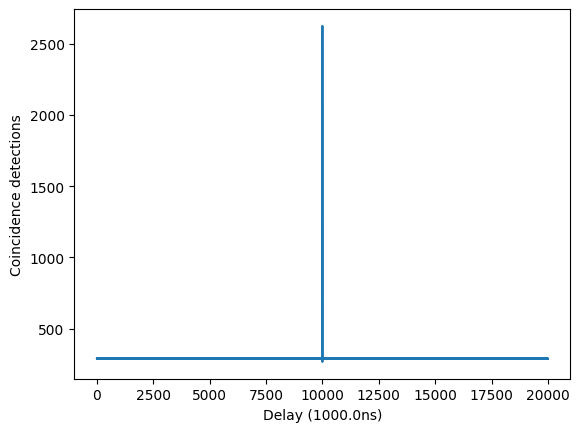
\includegraphics[height=4cm]{assets/unshifted_cc.png}
		\subcaption{}
	\end{subfigure}
	\begin{subfigure}[t]{0.49\textwidth}
		\centering
		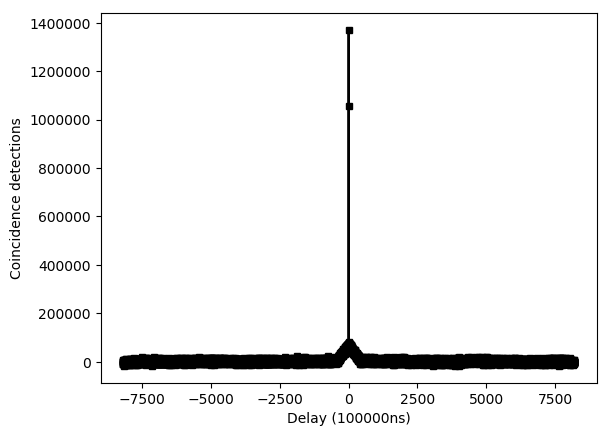
\includegraphics[height=4cm]{assets/firstDoppler_cc.png}
		\subcaption{}
	\end{subfigure}
	\caption{Autocorrelation of signal with (a) no shift (b) first order Doppler shift}
	\label{fig:firstDoppler_cc}
\end{figure}
\begin{figure}[ht!]
	\centering
	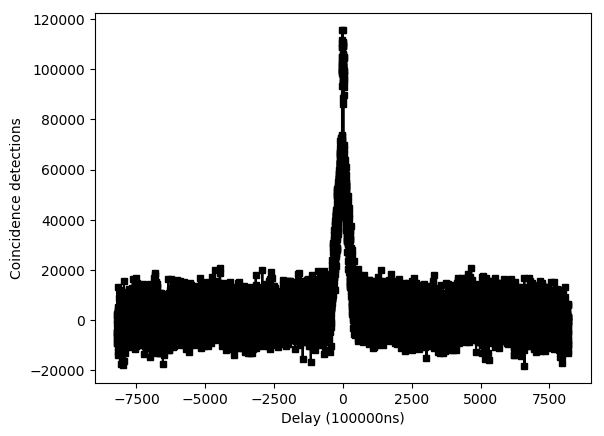
\includegraphics[width=0.95\linewidth]{assets/secondDoppler_cc.png}
	\caption{Autocorrelation of signal with first and second order Doppler shifts}
	\label{fig:secondDoppler_cc}
\end{figure}

\texttt{TODO: fill in machine learning method}

\begin{enumerate}
	\item find middle part with no shift
	\item try to shift middle part and find differential equation (order 2)
\end{enumerate}
 